\documentclass[12pt]{article}
\usepackage{wasysym} 
\usepackage{hyperref}
\usepackage{graphicx}
\usepackage{placeins}
\usepackage{epsfig}
\usepackage{epstopdf}
\usepackage{color}

\renewcommand{\familydefault}{\sfdefault}
\newcommand{\marker}[1]{Marker \color{red}\textbf{#1}\color{black}}

\title{\textbf{Dover War Memorial Project - User Guide}}
\date{}
\author{}
%%%%% document start
\begin{document}

\maketitle

\tableofcontents

\section{Introduction}

This document acts as a user guide for someone who will be also performing administration functions (i.e. it's not for the general public). It will identify features of each page, and how to perform all the actions required to maintain and update the website.

\section{Home Page \& Login}

\subsection{Home Page}
Figure~\ref{fig:home} shows the home page as viewed when not logged in.

\marker{1}\ links back to the home page, \marker{2}\ navigates to the Latest News area (Section~\ref{sec:siteUpdate}), \marker{3}\ to the Casualty Index (Section~\ref{sec:casualtyIndex}), \marker{4}\ to the Articles area (Section~\ref{sec:articles}), \marker{5}\ the Search area (Section~\ref{sec:search}) and \marker{6}\ to the Contact Us page. At the bottom of the page, these links are reproduced, with the addition of \marker{7}, which navigates to the Login page (Section~\ref{ssec:login}). These two menu bars appear on every page.

Other areas on the page are the latest news article (\marker{8}), the list of casualties who died today (\marker{9}) and the main narrative (\marker{10}).

\begin{figure}[h]
  \centering
 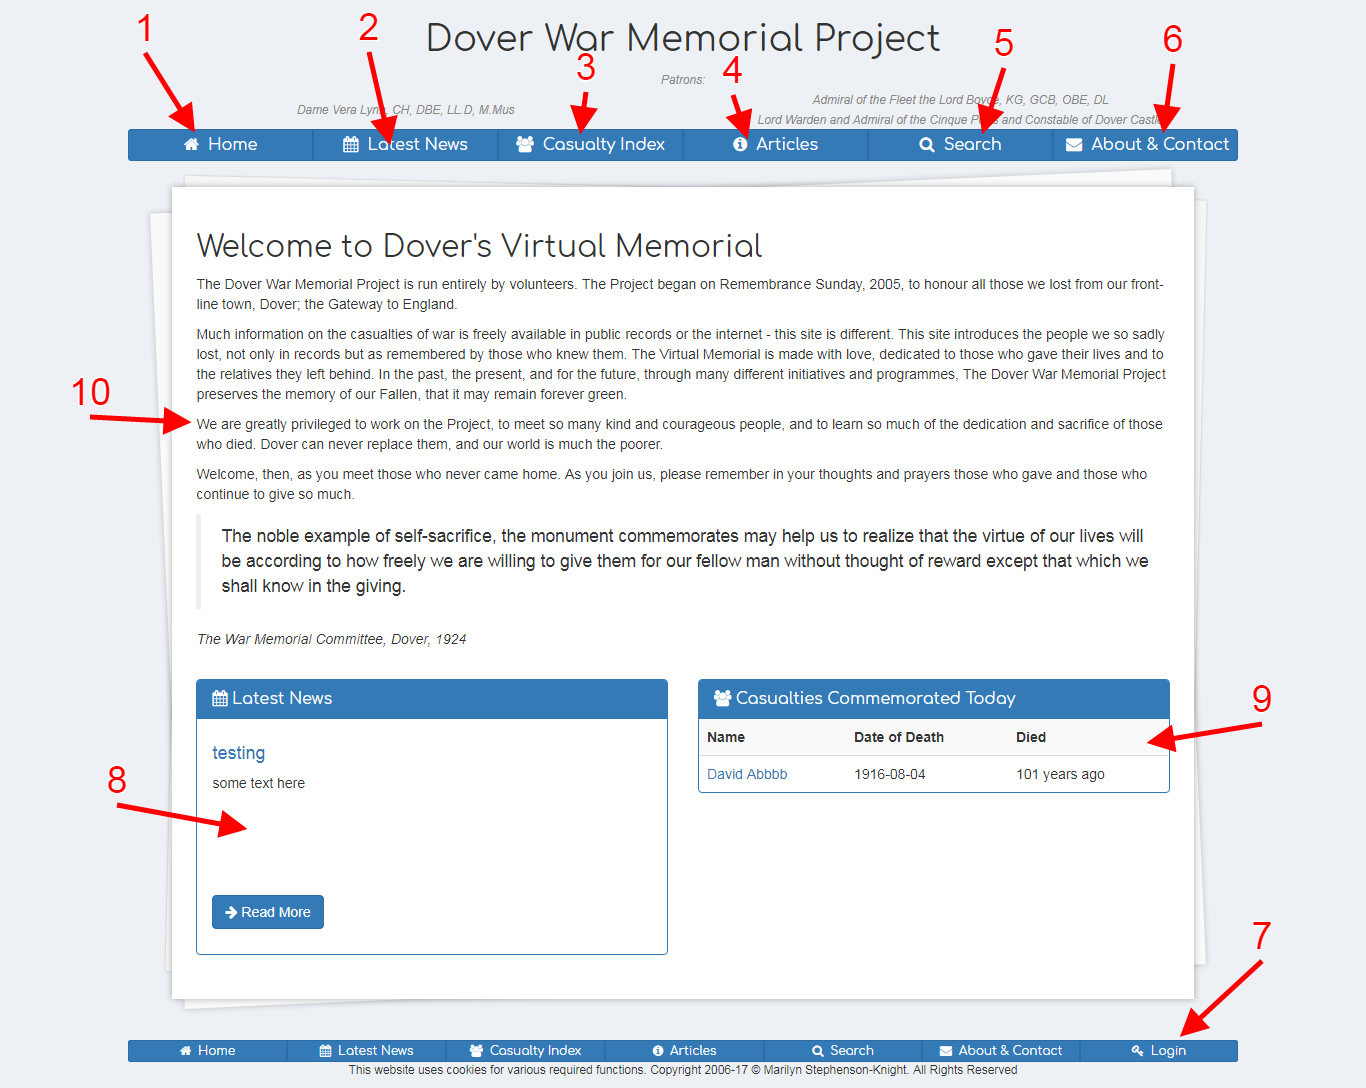
\includegraphics[width=\textwidth]{pics/home.png}
	\caption{Home Page}\label{fig:home}
\end{figure}

\FloatBarrier
\subsection{Login}\label{ssec:login}
This page (Figure~\ref{fig:login}) allows the user to login to the site to make various changes. \marker{1}\ is where the username must be entered with \marker{2}\ being the password field. \marker{3}\ submits this information.

\begin{figure}[h]
  \centering
 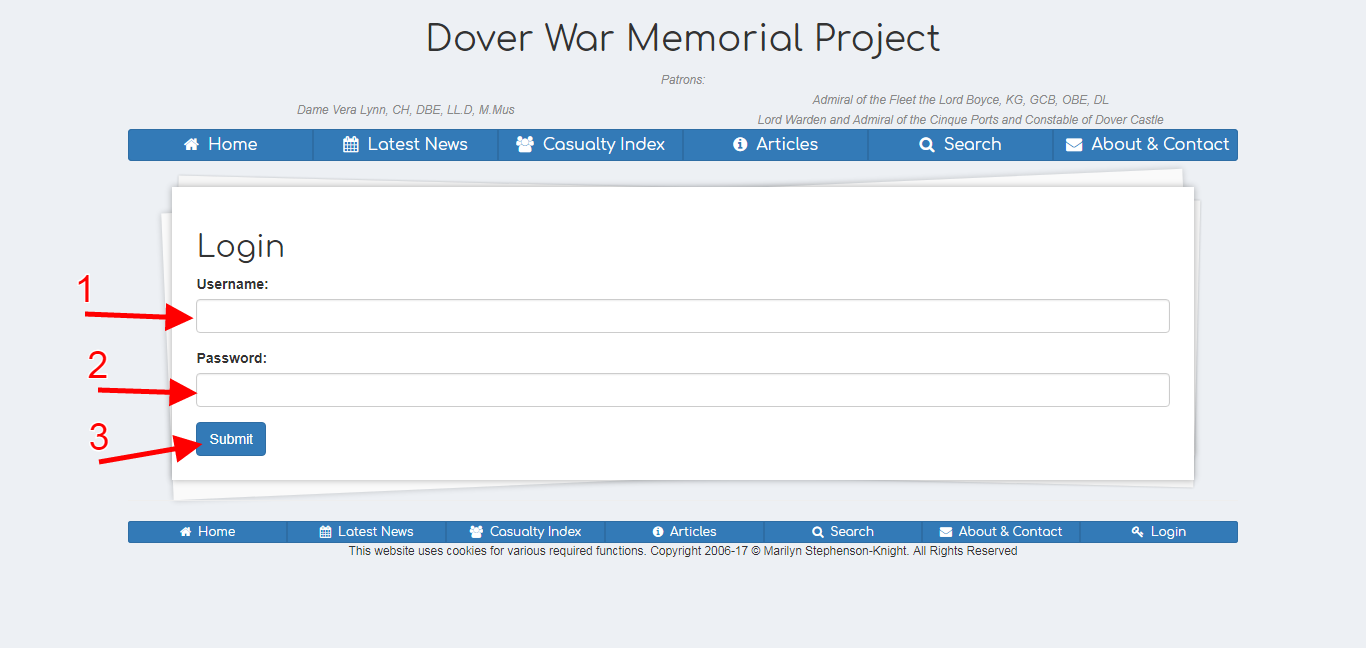
\includegraphics[width=\textwidth]{pics/login.png}
	\caption{Login Page}\label{fig:login}
\end{figure}

\FloatBarrier
\subsection{Home Page after Login}
Once a user has logged in, menu bars change. The top menu bar gains another row, with the login button on the bottom bar being replaced with a logout button, as can be seen in Figure~\ref{fig:home_login}. \marker{1}\ shows the currently logged in user, \marker{2}\ navigates to the config page (Section~\ref{sec:config}) and \marker{3}\ the admin help page (where this document is stored). \marker{4}\ and \marker{5}\ allow the user to logout. \marker{6} allows the user to edit the narrative text. These appear in numerous places across the site.

\begin{figure}[h]
  \centering
 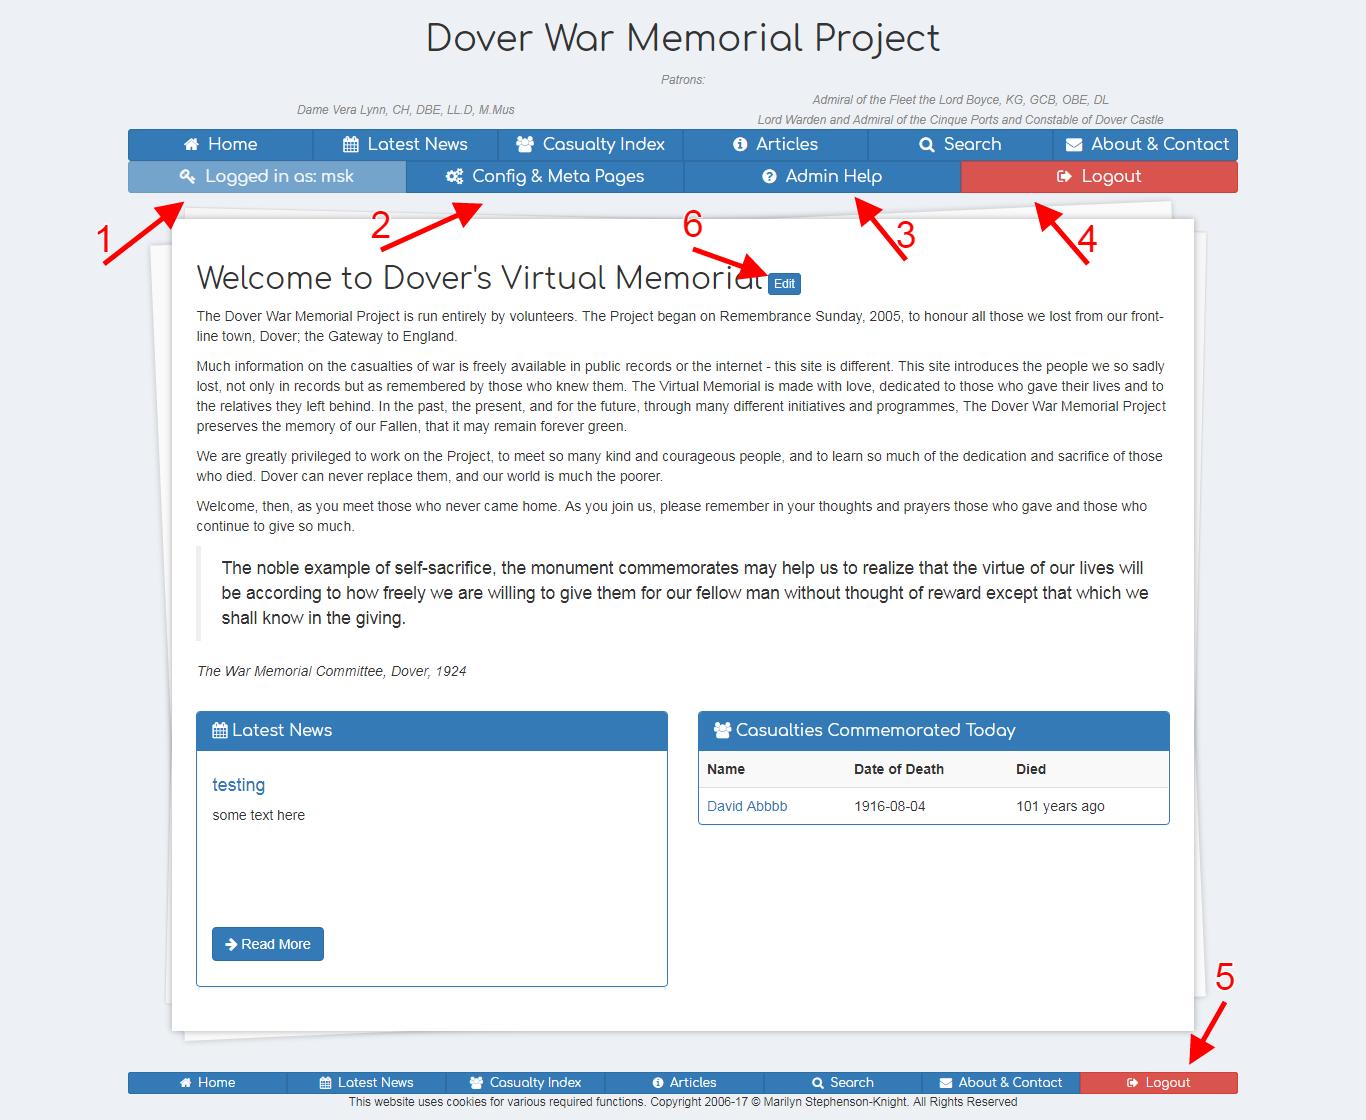
\includegraphics[width=\textwidth]{pics/home_login.png}
	\caption{Home Page after Login}\label{fig:home_login}
\end{figure}

\FloatBarrier
\section{Site Updates}\label{sec:siteUpdate}

\subsection{List Updates}
\subsection{View Update}
\subsection{Add / Edit Update}


\section{Casualty Index}\label{sec:casualtyIndex}

\subsection{List Memorials}
\subsection{Memorial Map}
\subsection{View Memorial}
\subsection{Add / Edit Memorial}
\subsection{View Casualty}
\subsection{View Casualty Data}
\subsection{Add / Edit Casualty}


\section{Articles}\label{sec:articles}
\subsection{View Article List}
\subsection{View Article}
\subsection{Add / Edit Article}

\section{Search}\label{sec:search}
\subsection{Text Search}
\subsection{Data Search}
\subsection{Search Results}

\section{Config \& Meta Pages}\label{sec:config}
\subsection{Meta Pages}
\subsection{List of Recently Uploaded Casualties}

\section{Others}
\subsection{Narrative Buttons}

\end{document}